\documentclass[12pt]{article}
\usepackage{graphicx}
\usepackage{Style-Thesis-Report}
\usepackage{wrapfig}
\usepackage{caption}
\usepackage{subcaption}

% You can define your own commands like this
\newcommand{\um}{$\upmu$m} % easily creates the label for ``micrometers''t

\begin{document} % Here is where the document begins
	
\begin{titlepage} 
\thispagestyle{empty}
	\begin{center}
	
\Huge
\textsc{McGill Physical Journal}
		\vspace*{1.5cm}
		
		\Huge
		\textbf{Measuring the Ratio of Specific Heats for Various Gases}
		\large
		\vspace{1.5cm}
		
		Joshua Manascu (260 870 343), Thomas Petuaud-Letang (Student ID)
	  % Add your names and student ID here
		
		McGill University Department of Physics
		
		\today
	\end{center}
		\hrule
	\begin{abstract} % This is the abstract. Replace the content with your own wording.
///
\end{abstract}
\hrule
\end{titlepage}
%\tableofcontents{}
%\thispagestyle{empty}
%\pagebreak
\setcounter{page}{1}
%The following commands will define header and footer
\rhead{McGill Physical Journal} % Do not change!
\lhead{Ratio of Specific Heats of a Gas}  % Add your lab title here
\cfoot{Page \thepage} % Do not change

\section{Introduction}\label{sec:introduction}
The \textit{Specific Heat} of a substance is the amount of energy which is required to raise a unit of the substance's mass by a degree of temperature. This is usually measured in $J Kg^{-1} K^{-1}$.
When dealing with a gas, we must also consider that the gas can expand. If it doesn't expand, then we can deal with the \textit{Specific Heat at Constant Volume} $C_v$. If, on the other hand, the gas expands and maintains a constant pressure when heat is supplied, then we are dealing with the \textit{Specific Heat at Constant Pressure} $C_p$. The latter quantity will be greater for any substance, because some of the energy contributes to the expansion of the gas as well as the increase in temperature.

Of particular interest is the ratio of these two quantities, the \textit{Ratio of Specific Heats}:
\begin{equation}\label{eq:gamma}
	\gamma = \frac{C_p}{C_v}
\end{equation}

This quantity is related to the internal structure of a gas' molecules, and can also be used to determine the speed of sound through the gas. $\gamma$ will be determined experimentally using two different methods.

\subsection{Method of Clément and Desormes}
In this method, the gas being tested is filled into a flask at slight above atmospheric pressure $H$ and allowed to reach a constant temperature. At this point the gas only occupies part of the flask.

\begin{figure}[h]
	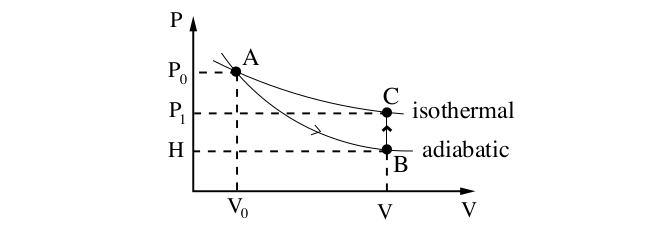
\includegraphics[width=1\textwidth]{Figures/Clement_Theory1}
\end{figure}
The stopper is then briefly removed and the gas expands to fill the entire flask, without the gas escaping or transferring heat with the outside. As a result of this sudden expansion, the gas will cool to below room temperature. We then allow it to heat back up to room temperature, thus increasing the pressure.



We can then determine $\gamma$ with:
\begin{equation}
	\gamma = \frac{\ln \left( \frac{P_0}{H} \right)}{\ln \left( \frac{P_0}{P_1} \right)}
\end{equation}

\subsection{Rüchardt’s Method}

\section{Procedure}
The flask is first flushed with the gas being tested to ensure no contamination of the results, and the pressure sensor is calibrated by noting the current atmospheric pressure $H$.

\subsection{Method of Clément and Desormes}
The following procedure was performed 10 times per gas tested so as to obtain 10 points of data per gas.

First, the flask was filled with the gas until the pressure reached somewhere in the range of 105 kPa to 115-120 kPa, which is the maximum the flask could handle before leaking. Once the pressure change had levelled, this was taken as thermal equilibrium and the value of $P_0$ was noted. For each run, $P_0$ was varied so that it would cover approximately the entire aforementioned range.

The flask was then briefly opened to allow the pressure to drop to $H$, and approximately 15-30 minutes was allowed to pass until the gas had warmed and the pressure change again levelled off. This value was then taken as $P_1$

\section{Results}
\subsection{Method of Clément and Desormes}
\begin{figure}[h]
	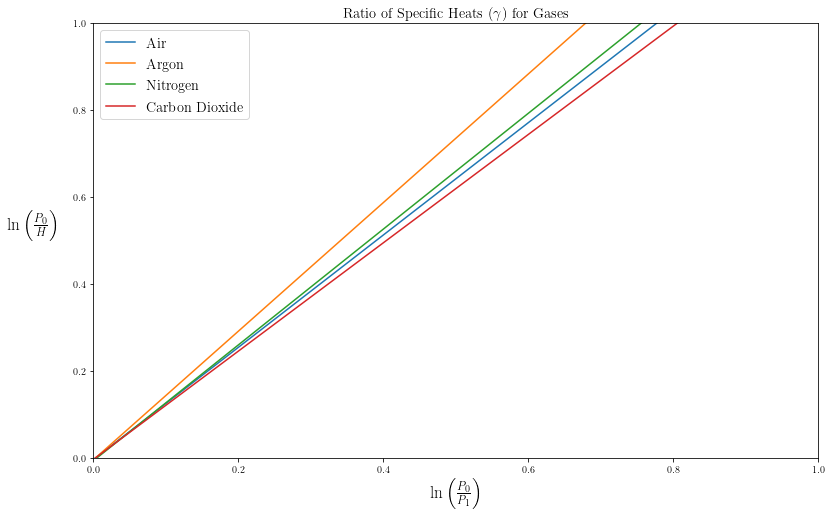
\includegraphics[width=1\textwidth]{Figures/Clement_All}
	\caption{Plot of linear fits of $\ln \left( \frac{{P_0}}{{H}} \right)$ vs $\ln \left( \frac{{P_0}}{{P_1}} \right)$ for every gas. A value for $\gamma$ can be extracted from the slope of the fit. See Appendix \ref{sec:AppendixA} for individual data points.}
\end{figure}
Above we see a plot of the linear fits for each gas, from which we can extract $\gamma$ as the slope (see Eq \ref{eq:gamma}). Using this and the uncertainty for the least squares fit, we can find:

\begin{center}
\begin{table}[H]	
\begin{tabular}{c | c | c}
	Gas & $\gamma$ from fit (kPa) & $\gamma$ from class data (kPa)\\
	\hline
	Argon & 1.48 $\pm$ 0.03 & 1.6 $\pm$ 0.4 \\
	Air & 1.29 $\pm$ 0.02 & 1.4 $\pm$ 0.3\\
	Nitrogen & 1.33 $\pm$ 0.02 & 1.2 $\pm$ 0.2\\
	Carbon Dioxide & 1.25 $\pm$ 0.01 & 1.3 $\pm$ 0.1\\
\end{tabular}
\caption{Value of $\gamma$ extracted from the fit and from the class data}
\end{table}
\end{center}

We also compared the $\gamma$ extracted from the fit with the gamma values calculated in the class data, of which there were 13 for each gas. These results are consistent with each other, within the range of their uncertainties.
\section{Discussion}
\subsection{Method of Clément and Desormes}
During data analysis, a fixed y-intercept value of 0 was considered as a first approximation for the linear fit. We compare that with a variable y-intercept for Nitrogen:
\begin{figure}[h]
	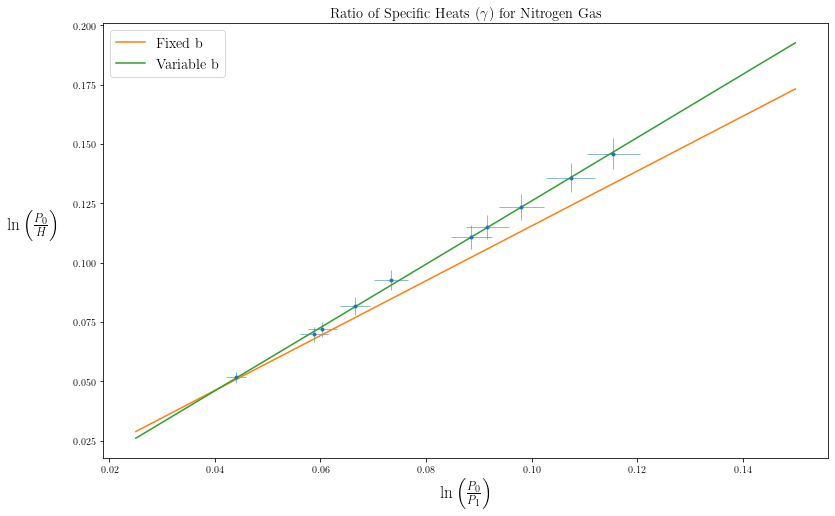
\includegraphics[width=1\textwidth]{Figures/Clement_N}
	\caption{Plot of $\ln \left( \frac{{P_0}}{{H}} \right)$ vs $\ln \left( \frac{{P_0}}{{P_1}} \right)$ for Nitrogen. A linear fit with a fixed and variable y-intercept are both considered.}
\end{figure}

The fixed b slightly underestimates the value of $\gamma$. This behaviour is consistent across the other three gases considered using this method (see Appendix \ref{sec:AppendixB}). For this reason, the standard linear fit with a variable b was used to extract the value of $\gamma$ for the collected data.

We compare that data to the accepted values:
\begin{center}
\begin{table}[H]
\begin{tabular}{c | c | c | c}
	Gas & Measured $\gamma$ (kPa) & Accepted $\gamma$ (kPa) & Percentage Error\\
	\hline
	Argon & 1.48 $\pm$ 0.03 & 5/3 & 11\%\\
	Air & 1.29 $\pm$ 0.02 & 7/5 & 7.7\%\\
	Nitrogen & 1.33 $\pm$ 0.02 & 7/5 & 4.8\%\\
	Carbon Dioxide & 1.25 $\pm$ 0.01 & 4/3 & 6.5\%\\
\end{tabular}
\caption{Measured value compared with the accepted values of $\gamma$ for various gases. The percentage error is also listed.}
\end{table}
\end{center}

The measured data seems to systematically underestimate the accepted value of $\gamma$ for the four gases. 

There are some aspects of this experiment that could lead to this. For one, the measurements of both $P_0$ and $P_1$ are done by eye, relying on the judgment of the experimenter to determine when equilibrium has been reached. It is very difficult to quantity the accuracy of these measurements beyond the base uncertainty of the pressure sensor. But if, for example, $P_1$ was consistently measured too quickly, that would lead to a lower $P_1$, and by extension, a lower $\gamma$. In addition, the theory assumes an ideal gas is present, but this is not necessarily true (and is definitely not true for air).
\section{Conclusions}
Using the method of Clément and Desormes, the value of $\gamma$ was determined , though it systematically underestimated the accepted values. In the future, it may be desirable to examine a single gas with a larger data set and in a more controlled environment (temperature, ambient pressure) to attempt a more accurate determination of $\gamma$
%\bibliographystyle{IEEEtran}
% Option 1 to create a bibliography is to use a .bib file.

% Option 2 is to add the bibliography manyally here.
%\begin{thebibliography}{2}
	%\bibitem{Brunner2013-longer} T. Brunner \textit{et al.} \textit{Trapped-ion decay spectroscopy towards the determination of ground-state components of $\beta\beta$ decay matrix elements}, Eur.Phys. J. A, 49(2013)142
		%\bibitem{Brunner2013-short} T. Brunner \textit{et al.} \textit{Trapped-ion decay spectroscopy towards the determination of ground-state components of $\beta\beta$ decay matrix elements}, Eur.Phys. J. A, 49(2013)142
	%%\bibitem{Brunner2013-short} more authors ,\textit{Journal}, volume(year)pages
	%%\bibitem{Brunner2013} Authors, \textit{Journal}(2010) 
	%%\bibitem{Sankey2010Strong} Sankey, J C and Yang, C and Zwickl, B M and Jayich, A M and Harris, J G E, \textit{Nature Physics} 9(2010)707
%\end{thebibliography}
%%%%%%%%% The appendix starts here. You can add tables, pictures, plots, graphs, data sets to your appendix.
\newpage
\appendix
\section{Appendix A}\label{sec:AppendixA}
\begin{figure}[h]
	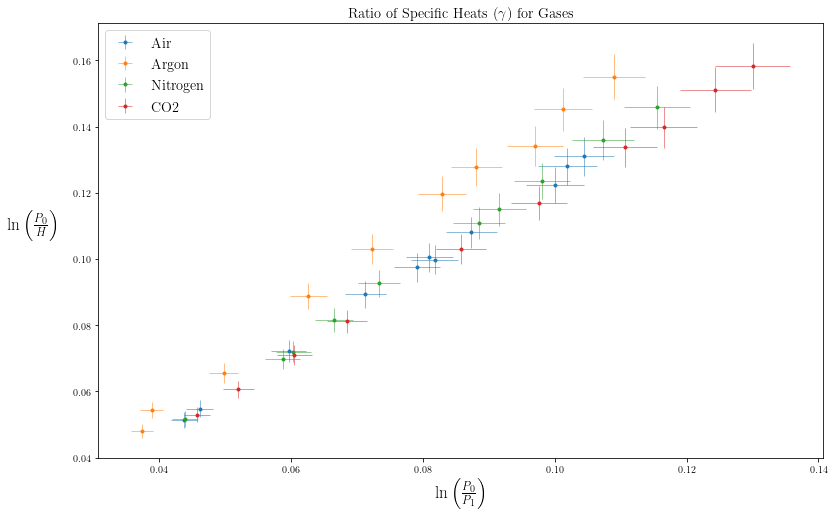
\includegraphics[width=1\textwidth]{Figures/Clement_All_points}
	\caption{Plot of $\ln \left( \frac{{P_0}}{{H}} \right)$ vs $\ln \left( \frac{{P_0}}{{P_1}} \right)$ for every gas. Uncertainties propagated from the uncertainty in the pressure sensor (0.01 kPa) and in the atmospheric pressure data (0.2 kPa).}
\end{figure}
\section{Appendix B}\label{sec:AppendixB}
\begin{figure}[H]
	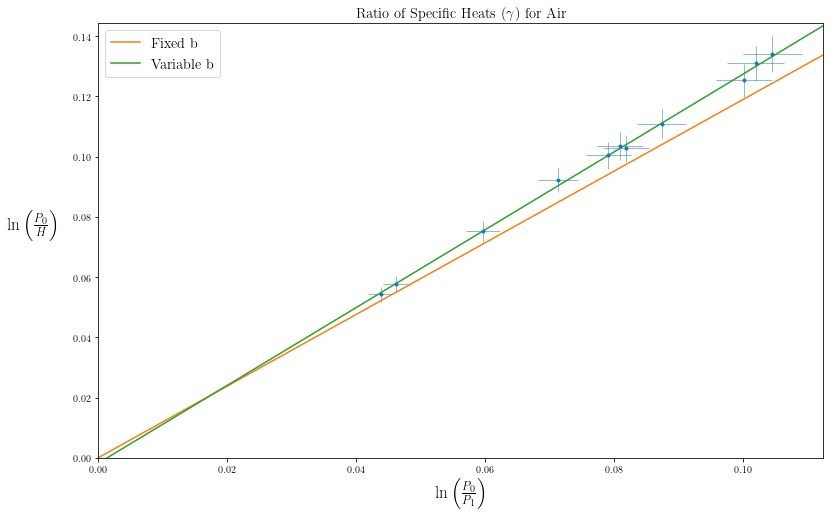
\includegraphics[width=0.7\textwidth]{Figures/B_Air}
		\caption{Plot of $\ln \left( \frac{{P_0}}{{H}} \right)$ vs $\ln \left( \frac{{P_0}}{{P_1}} \right)$ for Air. A linear fit with a fixed and variable y-intercept are both considered.}
\end{figure}

\begin{figure}[H]
	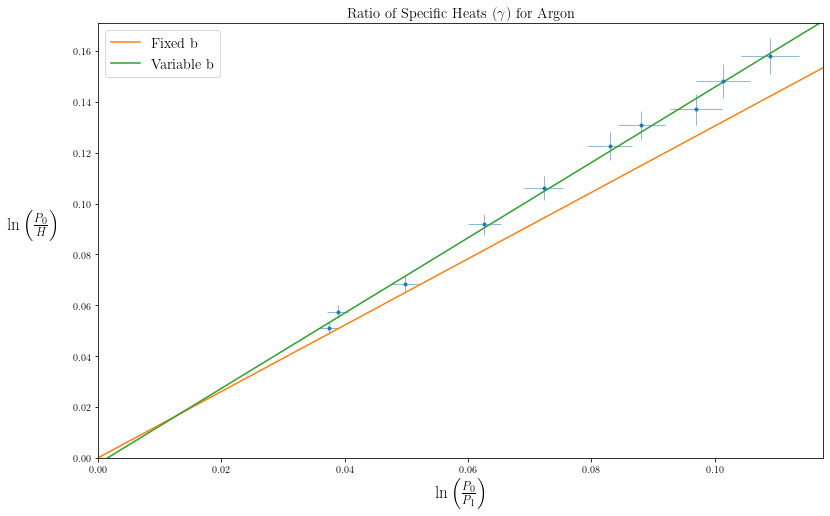
\includegraphics[width=0.7\textwidth]{Figures/B_Argon}
	\caption{Plot of $\ln \left( \frac{{P_0}}{{H}} \right)$ vs $\ln \left( \frac{{P_0}}{{P_1}} \right)$ for Argon. A linear fit with a fixed and variable y-intercept are both considered.}
\end{figure}

\begin{figure}[H]
	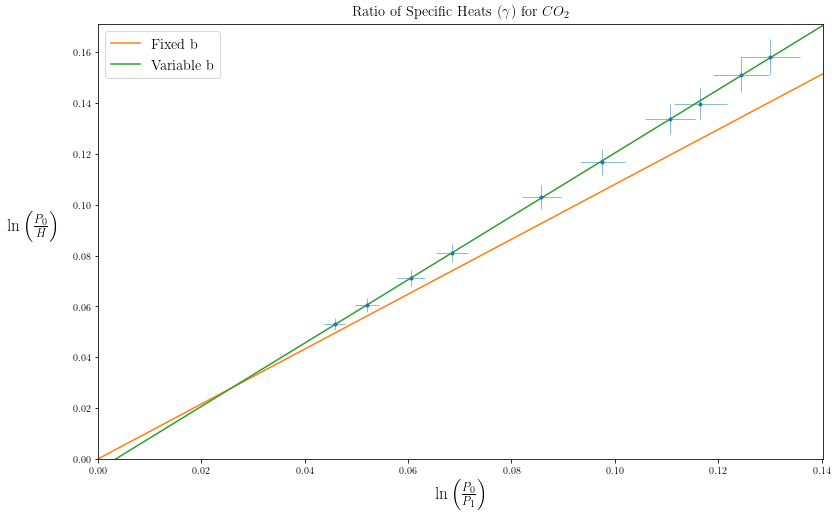
\includegraphics[width=0.7\textwidth]{Figures/B_CO2}
	\caption{Plot of $\ln \left( \frac{{P_0}}{{H}} \right)$ vs $\ln \left( \frac{{P_0}}{{P_1}} \right)$ for $CO_2$. A linear fit with a fixed and variable y-intercept are both considered.}
\end{figure}
\end{document}
%%%%%%
% McGil logo from McGill webpage
% Note: atom logo from http://images.google.de/imgres?imgurl=https%3A%2F%2Fupload.wikimedia.org%2Fwikipedia%2Fcommons%2Fthumb%2F8%2F80%2FAtom_editor_logo.svg%2F2000px-Atom_editor_logo.svg.png&imgrefurl=https%3A%2F%2Fcommons.wikimedia.org%2Fwiki%2FFile%3AAtom_editor_logo.svg&h=1832&w=2000&tbnid=Pu9l8_1ca47MzM%3A&vet=1&docid=DMy5AX000LwZRM&ei=bmZqWO-xL-mRgAaFlrGgCw&tbm=isch&iact=rc&uact=3&dur=2247&page=0&start=0&ndsp=18&ved=0ahUKEwjvoP_L2KPRAhXpCMAKHQVLDLQQMwgcKAIwAg&safe=off&bih=634&biw=1141